\chapter{Tau Lepton Final State Separation}
\label{chap:Tau}

\chapterquote{MVA: Turn numbers into gold.}%
{TMVA}%: Blackwood's Magazine May 1830


\section{Introduction}

Why study tau

% TODO tau life time
Tau lepton has been examined closely in the past. The decay and the spin of the decay product were direct tests to the standard model. The spin of the decay product, using a Higgs decaying to tau tau channel, allows one to determine the spin of the higgs. Also, as tau is short-lived, only its decay products can be detected and reconstructed in the detector. Therefore, the ability to reconstruct and separate different tau decay modes is benchmark of detector performances.

\section{Analysis}

This chapter will describe a tau final decay separation study. The processor developed for the study is used to test different detector models, as a proof-of-principle of detector optimisation using tau decay separation. Lastly, the spin of the higgs was studied using one higgs decaying to two tau tau channel.


\section{Simulation and reconstruction}

\eeToTauTau channel is used for the tau decay mode separation study. Generator software WHIZARD 1.95 \cite{whizard} is used to generated simulated Monte Carlo (MC) samples. Hadronisation is described with PYTHIA 6.4 \cite{Sjostrand:1995iq}, which is tuned to the LEP results \cite{}. The spin effect of tau lepton decay is described by TAUOLA \cite{Jadach:1993hs}.

Final state radiation (FSR) was simulated. The initial state radiation (ISR) and the beam induced background were not simulated.

Events were simulated with the \CLICILD detector concept, using software with MOKKA \cite{MoradeFreitas:2002kj}, based on the GEANT 4 package  \cite{Agostinelli:2002hh}.
Events were reconstructed with  ilcsoft version v01-17-07 \cite{Gaede:82475} and PandoraPFA version v02-02-00 \cite{Marshall:2015rfa}, where the photon reconstruction is described in \cite{Xu:2016rcz}.

\section{Generator level cut}

To study the difference between different tau decay modes, clear topological difference is required. Therefore, events was considered if the event passes a set of cuts at generator level, listed here
\begin{itemize}
  \item the final state photons not converting to electron pair in the tracker,
  \item the tau leptons decaying in the barrel and the end cap regions, which are defined as polar angle between 0.3 to 0.6 rad and 0.8 to 1.57 rad, and
  \item the visible energy of the tau lepton decay products more than 5\,GeV, where the visible energy of the tau lepton decay is defined as the energy of the tau minus the energy of the tau neutrino.
\end{itemize}

The angular requirement is due to the gap region between the barrel and and the end cap of calorimeters, which degrades the PFO resolution significantly.

Around two million events were simulated for this study.


\section{Decay modes}

\begin{table}[htbp]
\centering
\caption{\label{tab:TauDecayMode} Branching ratios of the seven major \Pgtm decays, taken from \cite{Agashe:2014kda}. \Pgtp decays similarly to \Pgtm.}
\smallskip
\begin{tabular}{|l |r|}
\hline
  \textbf{Decay final state} & \textbf{Branching ratio / \%} \\
\hline
  \decayElectron        & 17.83$\pm$0.04   \\
  \decayMuon  	& 17.41$\pm$0.04  \\
  \decayPion     	& 10.83$\pm$0.06   \\
  \decayRho	& 25.52$\pm$0.09 \\
  \decayAiPhoton	& 9.30$\pm$0.11    \\
  \decayAiPion  	    & 8.99$\pm$0.06  \\
  \decayThreePionPhoton  	    & 2.70$\pm$0.08  \\

\hline
\end{tabular}
\end{table}

Seven major decay final states of the tau lepton shown in \Table{tab:TauDecayMode} were studied, covering 92.58\,\% of all tau decays  \cite{Agashe:2014kda}.  Decay modes not listed in the table have branching fractions lower than 1\% each. These final states can be classified into three categories: leptonic decays (\decayElectron and \decayMuon), one-prong with photons (\decayPion, \decayRho and \decayAiPhoton), and three-prong with photons (\decayAiPion and \decayThreePionPhoton).

The studied channel, \eeToTauTau, contains two \Pgt decaying in opposite directions. To select decay products of one \Ptau, the fiducial detector space was divided into two halves. %This is possible because ISR and beam induced background was not simulated.
Event shape variable thrust is used to separate two halves. The classical event shape thrust\cite{PhysRevLett.39.1587}, is defined as
\begin{equation}
T = \max_{\hat{t}}\!\frac{\sum_{i}\absOf{\hat{t}\!\cdot\!\vec{p_{i}}}}{\sum_{i}\absOf{\vec{p_{i}}}}
\end{equation}
where $\vec{p_{i}}$ is the momentum vector of the particle $i$. Summation is over all particles in the event. Thrust axis, $\hat{t}$, is a unit vector. (Principle) Thrust value, $T$, is 1 for a perfect pencillike back-to-back two-jet event, and 0.5 for a perfect spherical event. The sign of dot product between thrust axis and PFO momentum determines which half the PFO falls into.


\section{Discriminative varibles}

\begin{figure}[htbp]
\centering
% \begin{center}/\end{center} takes some additional vertical space

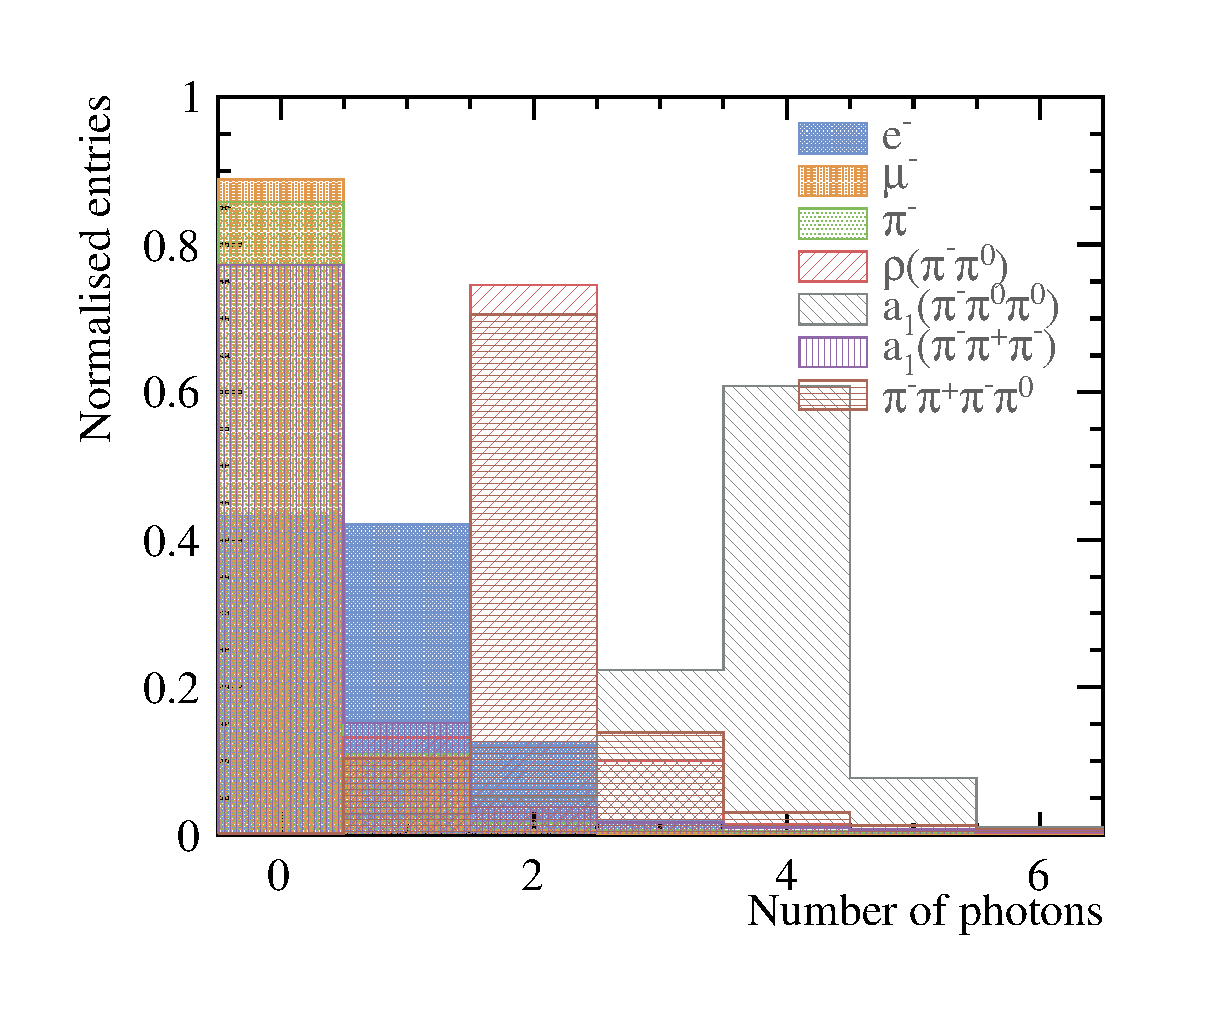
\includegraphics[width=.45\textwidth]{tau/var/nPhoton_100GeV_improved}
\qquad
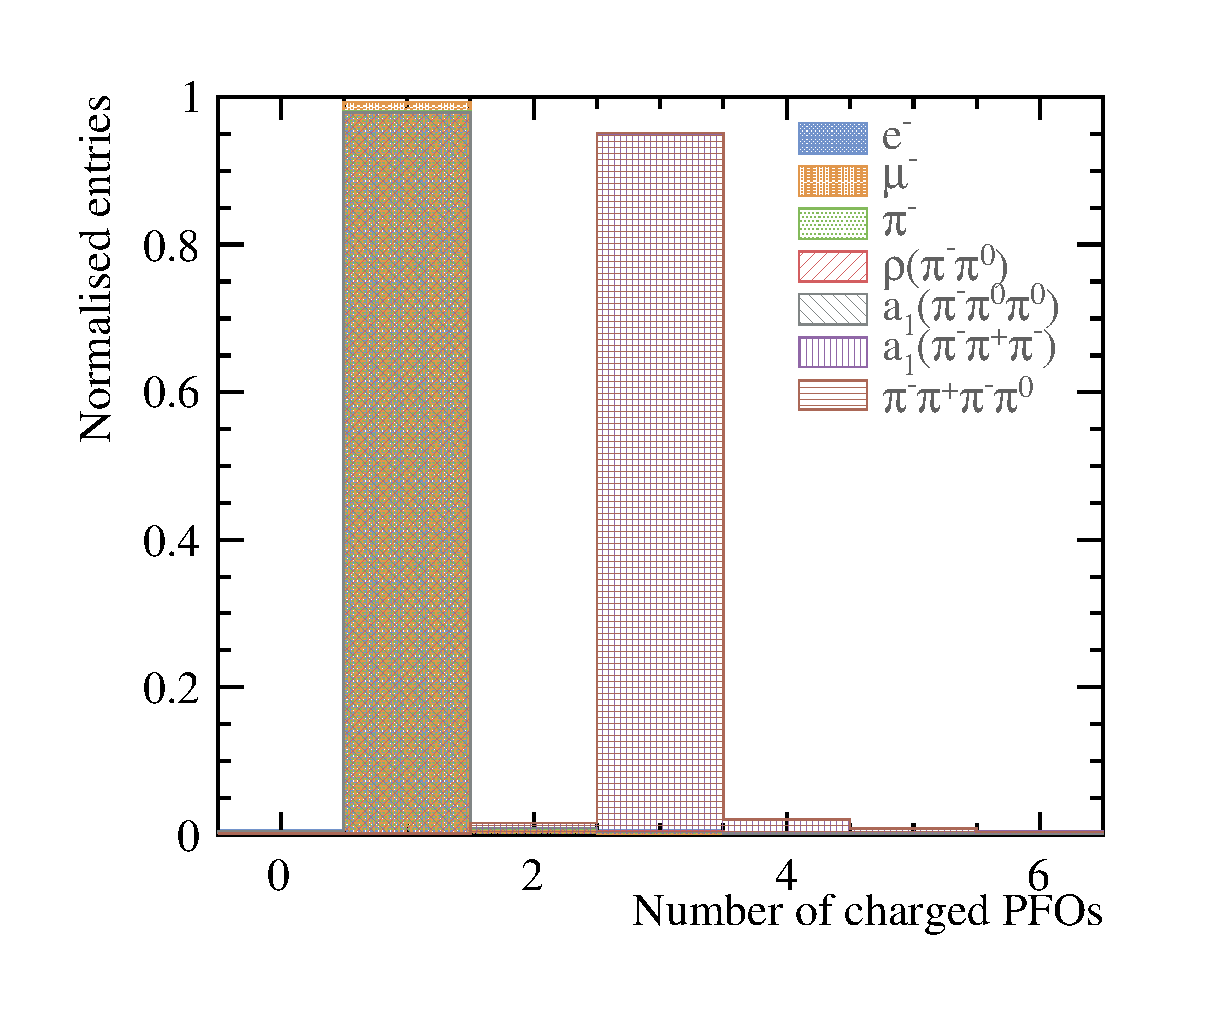
\includegraphics[width=.45\textwidth]{tau/var/nCharge_100GeV_improved}
\qquad
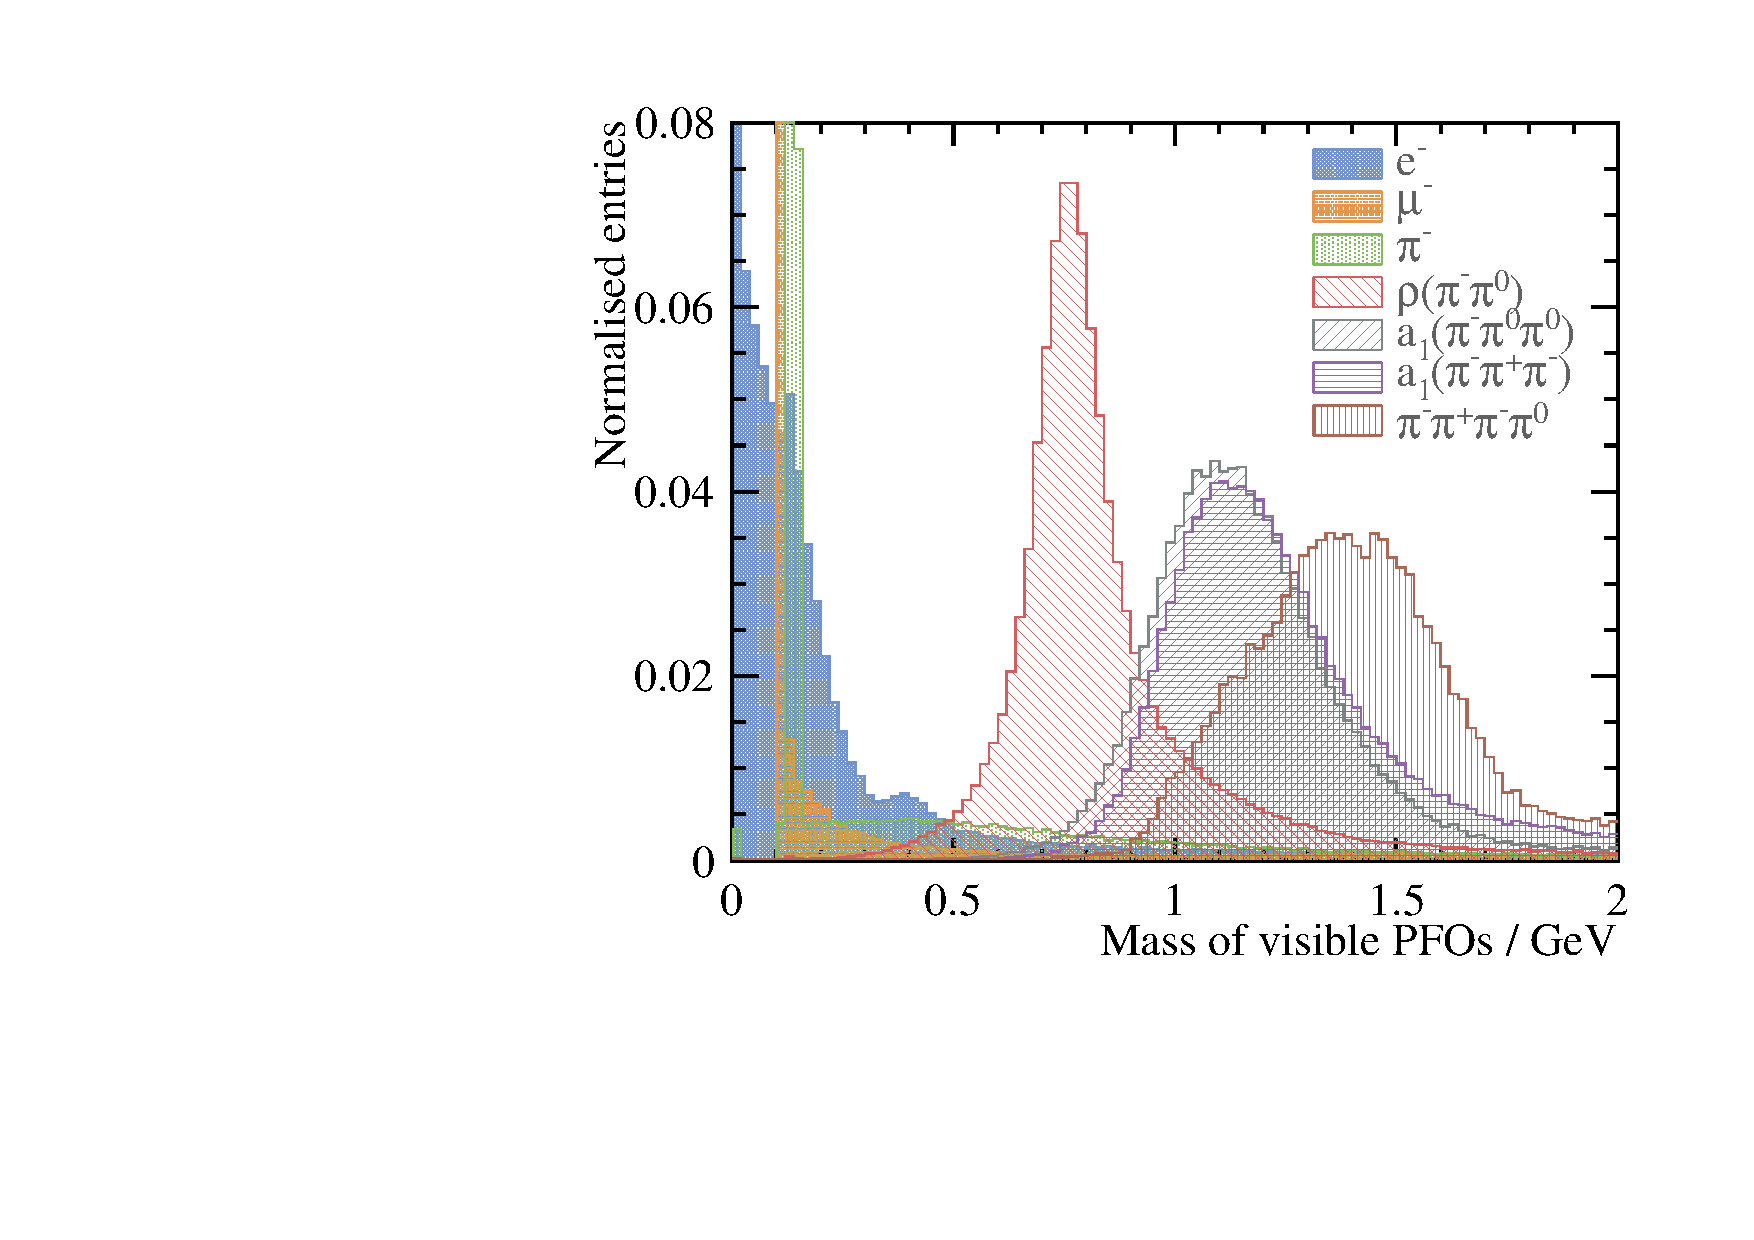
\includegraphics[width=.45\textwidth]{tau/var/mVis_100GeV_improved_zoom}
\qquad
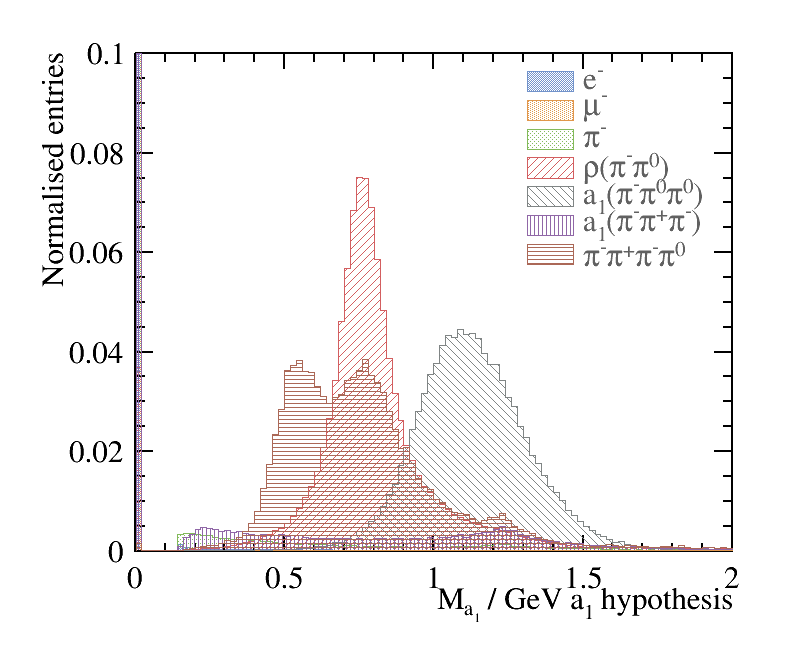
\includegraphics[width=.45\textwidth]{tau/var/mA1A1Fit_100GeV_improved_zoom}
\qquad

\caption[]{
Normalised distribution for selected discriminative variables for seven final states, \decayElectron, \decayMuon, \decayPion, \decayRho, \decayAiPhoton, \decayAiPion and \decayThreePionPhoton, separated using truth information,  for \rootSGeV{100} for nominal \CLICILD detector model. The top left, top right, bottom left and bottom right plots are the normalised entries against the number of photons, number of charged PFOs, invariant mass of visible PFOs, and the invariant mass of \decayAiPhotonShort for hypothesis test, respectively. There is a clear distinction between different final states in each plot.
}
\label{fig:tauVar}
\end{figure}

Some variables with most discriminative power are shown in figure~\ref{fig:nPfos}. In total 29 variables used in the multivariate analysis. The reason for the large number of variables is due to training seven decay modes at once, which will be discussed later.

Here is a full list of all variables used in the multivariate analysis.

\begin{itemize}
\item  $\frac{E_{ECal,HCal}}{E_{tot}}, charged$:  Sum of energy deposited in ECal and HCal, divided by the energy of charged particles
\item  $\frac{E_{ECal,HCal}}{E_{tot}}, all$:  	 Sum of energy deposited in ECal and HCal, divided by the energy of all particles
\item  $m_{vis}$:     	 Invariant mass of visible particles in GeV
\item  $\frac{E_{vis}}{E_{\Ptauon}}$:	 Sum of energy of all particles, divided by the energy of \Ptauon
\item  $\frac{E_{charged}}{E_{\Ptauon}}$:	 Sum of energy of charged particles, divided by the energy of \Ptauon
\item  $\frac{E_{\Pgmm}}{E_{\Ptauon}}$:	 Sum of energy of muons, divided by the energy of \Ptauon
\item  $\frac{E_{\Pem}}{E_{\Ptauon}}$:	 Sum of energy of electrons, divided by the energy of \Ptauon
\item  $\frac{E_{\Pgg}}{E_{\Ptauon}}$:	 Sum of energy of photons, divided by the energy of \Ptauon
\item  $\frac{E_{\Pgpm}}{E_{\Ptauon}}$:	 Sum of energy of charged pions, divided by the energy of \Ptauon
\item  $N_{charged}$:	 Number of charged particles
\item  $N_{\Pgmm}$:	 Number of muons
\item  $N_{\Pem}$:	 Number of electrons
\item  $N_{\Pgg}$:	 Number of photons
\item  $N_{\Pgpm}$:	 Number of charged pions
\item  $m_{\Pgg}$:     	 Invariant mass of photons in GeV
\item  $m_{charged}$:     	 Invariant mass of charged particles in GeV
\item  $m_{neutral}$:     	 Invariant mass of neutral particles in GeV
\item  $m_{\Pgpm}$:     	 Invariant mass of charged pions in GeV
\item  $m_{\Pgpz}, \decayRhoShort hypothesis$:     	 Fitted invariant mass of \Pgpz for \decayRhoShort hypothesis test
\item  $m_{\decayRhoShort}, \decayRhoShort hypothesis$:     	 Fitted invariant mass of \decayRhoShort for \decayRhoShort hypothesis test

\item  $m_{\Pgpz1}, \decayAiPhotonShort hypothesis$:     	 First fitted invariant mass of \Pgpz, for \decayAiPhotonShort hypothesis test, ordered by closeness to the true \Pgpz mass
\item  $m_{\Pgpz2}, \decayAiPhotonShort hypothesis$:     	 Second fitted invariant mass of \Pgpz, for \decayAiPhotonShort hypothesis test, ordered by closeness to the true \Pgpz mass
\item  $m_{\decayAiPhotonShort}, \decayAiPhotonShort hypothesis$:     	 Second fitted invariant mass of \decayAiPhotonShort, for \decayAiPhotonShort hypothesis test
\item  $\bar{E_{cell}}$:     	 Average energy deposited in a calorimeter cell in GeV
\item  $d_{trans,shower}$:    Transverse shower width for electromagnetic shower profile, averaged for all clusters in the ECal
\item  $l_{long,shower}$:    Longitudinal start layer for electromagnetic shower profile, averaged for all clusters in the ECal
\item  $\Delta{l_{long,shower}}$:    Longitudinal discrepancy for electromagnetic shower profile, averaged for all clusters in the ECal
\item  $\%MIP$:    Fraction of calorimeter hits registered as minimum ionised particles, averaged for all clusters in the ECal
\item  $\frac{E}{P}$:   Energy divided by momentum, averaged for all clusters in the ECal
\end{itemize}

Number of photons is an important variable for separating decay modes. This information is only available due to the excellent photon reconstruction. Shown in \Figure{fig:nPfos}, the majority of \decayMuon, \decayPion and \decayAiPion final states have zero photon reconstructed. The \decayElectron final state event have one photon reconstructed instead of zero, due to the FSR effect. \decayRho and \decayThreePionPhoton have nearly 80\% events with two reconstructed photons, whilst \decayAiPion have over 60\% events with four reconstructed photons. The loss is efficiency is due to the increasing difficulty to separate nearby photons.

The number of charged PFOs can clearly separate the leptonic and 1-prong final states, from the 3-prong final states, shown in \Figure{fig:nPfos}. The efficiency of leptonic final states are over 98\%.

The invariant mass of the visible PFOs shows clear differences between different final states. \decayRho, \decayAiPhoton and \decayAiPion distribution show clear resonance at \Prho and \Pai. \decayElectron, \decayMuon and \decayPion distribution show much smaller invariant mass and \decayThreePionPhoton shows a large invariant mass than \Pai. The \decayElectron final state has a long tail of invariant mass due to the extra photons from the FSR.



